\section{Running \CNAME\label{sec:RunningCasal2}\index{Running \CNAME}}

\CNAME\ is run from a console window (i.e., the command line) on \I{Microsoft Windows} or from a terminal window on \I{Linux}. \CNAME\ uses information from input data files -{}- the \emph{\config\index{Input configuration file}}\ being the input file that is supplied to \CNAME.

The \config\ is required and defines the model structure, processes, observations, parameters (both the fixed parameters and the parameters to be estimated)\index{Estimable parameters}, and the requested reports (outputs).

By convention, the name of the \config~ ends with the suffix \texttt{.csl2}. However, any suffix is acceptable. The default name for the \config~ is \emph{config.csl2} and if used it does not have to be specified as one of the command line arguments to to \CNAME. Note that the \config\ can include other separate files so the specification can be split into digestible parts. 

Command line arguments\index{Command line arguments} are used to specify the actions or \emph{tasks}\index{Tasks} of \CNAME, e.g., to run a model with a set of parameter values, to estimate parameter values (either point estimates or MCMC), to project quantities, or to simulate observations.For example, \texttt{-r} is the \emph{run} mode, \texttt{-e} is the \emph{estimation} mode, and \texttt{-m} is the \emph{MCMC} mode. The \emph{command line arguments} are described in Section \ref{sec:CommandLineArguments}.

\subsection{\I{Using \CNAME}}

To use \CNAME, open a console window (i.e. the command prompt) window on Microsoft Windows or a terminal window on Linux. Navigate to the directory where the model \config s are located. Then enter \cname~with arguments for a specific mode to start the \CNAME mode running; see Section \ref{sec:CommandLineArguments} for the list of possible arguments. \CNAME\ will print output to the screen.

For both 64-bit Linux and Microsoft Windows, we recommend using the install package available on \github\ for Microsoft Windows or the Debian package (.deb) for Linux. Running \CNAME\ on a system requires the main binary (casal2.exe on Windows, or casa2 on Linux) and the associated dynamically linked libraries (DLL) for Windows or shared objects (.so) for Linux to be installed into appropriate directories, and cannot be (easily) run by copying the binary to a working directory. \CNAME\ is not available for 32-bit operating systems or macOS.

\subsection{\I{Redirecting standard output}\label{sec:RedirectingStandardOut}}

\CNAME\ uses the \texttt{standard output}\index{standard output} stream to display runtime information. The \I{standard error} stream is used by \CNAME\ to output the program exit status and runtime errors. We suggest redirecting both the standard output and standard error into an appropriate file or files\index{Redirecting standard out}\index{Redirecting standard error}.

With the bash shell (on Linux systems), you can do this using the command structure

\begin{verbatim} (casal2 [arguments] > run.out) >& run.err &\end{verbatim}

It may be useful to redirect the standard input, especially if you're using \CNAME\ inside a batch job, i.e.

\begin{verbatim} (casal2 [arguments] > run.out < /dev/null) >& run.err &\end{verbatim}

On Microsoft Windows systems, you can redirect to standard output using

\begin{verbatim} casal2 [arguments] > run.out\end{verbatim}

And, on some Microsoft Windows systems (e.g., Windows 10), you can redirect to both standard output and standard error, using the syntax

\begin{verbatim} casal2 [arguments] > run.out 2> run.err\end{verbatim}

\CNAME\ outputs header information to the output (Figure~\ref{fig:log_file_1}). The header\index{Output header information} consists of the program name and version, the arguments passed to \CNAME\ from the command line, the date and time that the program was called (derived from the system time), the user name, and the machine name (including the operating system and the process identification number). This information can be used to track outputs as well as identifying the version of \CNAME\ used to run the model.

\begin{figure}[htp]
	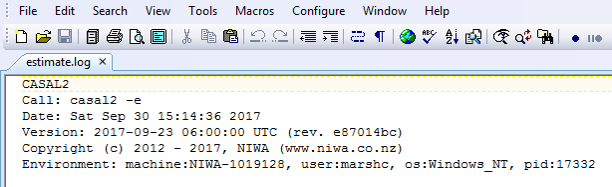
\includegraphics[scale=1]{Figures/eglog.png}
	\caption{\textbf{Example of output file header information.}}\label{fig:log_file_1}
\end{figure}

\vspace*{4mm}

\subsection{\I{Command line arguments}\label{sec:command-line-arguments}}

\CNAME~is called using:

\texttt{\cname [-c \emph{config\_file}] [\emph{task}] [\emph{options}]}

where

\begin{description}
  \item [\texttt{-c \emph{config\_file}}] Define the \config~for \CNAME\ (if this argument is omitted, the default \config~is \texttt{config.csl2})
\end{description}

and where \emph{task} must be one of the following (\textbf{[]} indicates a secondary label to call the task, e.g. \textbf{\texttt{-h}} will execute the same task as \textbf{\texttt{-{}-help}}),

\begin{description}
\item [\texttt{-h [-{}-help]}] Display help (this page)
\item [\texttt{-l [-{}-licence]}] Display the reference for the software license (GPL v2)
\item [\texttt{-v [-{}-version]}] Display the \CNAME~version number

\item [\texttt{-r [-{}-run]}] \emph{Run} the model once using the parameter values in the \config, or optionally with the parameter values from the file specified with argument \texttt{-i \emph{filename}}

\item [\texttt{-e [-{}-estimate]}] Do a point \emph{estimate} using the values in the \config~as the starting point for the parameters to be estimated, or optionally with the starting parameter values from the file specified with the argument \texttt{-i \emph{filename}}.

\item [ \texttt{[-{p}-profiling]}] Do a likelihood \emph{profile} using the parameter values in the \config~as the starting point, or optionally with the starting parameter values from the file specified with the argument \texttt{-i \emph{filename}}

\item [\texttt{-m [-{}-mcmc]}] Do an \emph{MCMC} chain. The the co-variance matrix is first estimated using the values in the \config~as the starting point for the parameters to be estimated, or optionally with the starting parameter values from the file specified with the argument \texttt{-i \emph{filename}}. Use \texttt{--skip-estimation} to skip estimating the co-variance matrix and to read it in from a file.

\item [\texttt{-f [-{}-projection]}] \emph{arg}. Project the model \emph{forward} in time using the parameter values in the \config~as the starting point for the estimation, or optionally with the parameter values from the file specified with the argument \texttt{-i \emph{filename}}. Repeat each parameter set \emph{arg} times (default 1). Normally, the MCMC sample are used via \texttt{-i}

\item [\texttt{-s [-{}-simulation]} \emph{number}] \emph{Simulate} the \emph{number} of observation sets using values in the \config~as the parameter values, or optionally with the parameter values from the file specified with the argument \texttt{-i \emph{filename}}
\end{description}

and where the following optional arguments\index{Optional command line arguments} [\emph{options}] may be specified

\begin{description}
\item [\texttt{-i [-{}-input] \emph{filename}}] \emph{Input} one or more sets of free (estimated) parameter values from \texttt{\emph{filename}} (see Section \ref{sec:report-syntax} for details about the format of \texttt{\emph{filename}})

\item [\texttt{-o [-{}-output]\emph{filename}}] \emph{Output} a report of the free (estimated) parameter values in a format suitable for \texttt{-i \emph{filename}} (see Section \ref{sec:report-syntax} for details about the format of \texttt{\emph{filename}})

\item [\texttt{-g [-{}-seed]\emph{seed}}] Initialise the random number \emph{generator} with \texttt{\emph{seed}}, a positive (long) integer value (note, if \texttt{-g} is not specified, then \CNAME~will  generate a random number seed based on the computer clock time)

\item [\texttt{-{}-loglevel}] arg = \{trace, finest, fine, medium\} (see Section \ref{sec:Report})

\item [\texttt{-{}-tabular}] Run with \texttt{-r} or \texttt{-f}  command to print \command{report} in tabular format (see Section \ref{sec:report-section})

\item [\texttt{-{}-single-step}] Run with \texttt{-r} to pause the model and ask the user to specify parameters and their values to use for the next iteration (see Section \ref{sec:singlestepping})

\item [\texttt{   [-{}-resume] }] Resume a MCMC chain

\item [\texttt{   [-{}-objective-file] }] \emph{arg}. Objective file for resuming an MCMC is \emph{arg}

\item [\texttt{   [-{}-sample-file] }] \emph{arg}. Sample file for resuming an MCMC is \emph{arg}

\item [\texttt{   [-{}-skip-estimation] }] For \texttt{   [-{}-mcmc]} run, skip estimating the covariance matrix; take it from the file \texttt{mpd.out}. This is a way use a re-calculated covariance matrix based on a previous MCMC run and start a new chain

\item [\texttt{   [-{}-no-mpd] }] For \texttt{-e   [-{}-estimate]} run, do not create the MPD file, \texttt{mpd.out}

\item [\texttt{-q [-{}-query]\emph{object type}}] \emph{Query} an object type to print an extract of the object description and parameter definitions.  An object can be defined as \texttt{\emph{block.type}}, e.g. \texttt{casal2 -{}-query process.recruitment\_constant} will query the constant recruitment block.

\end{description}

\subsection{Constructing the \CNAME~\config s \label{constructing-config}}\index{Input configuration file syntax}

By convention, the \config~is a stub that names four other files that cover four broad sections:

\begin{itemize}
	\item the description of the population structure, dynamics, and parameters (\texttt{population.csl2},Section \ref{sec:population-section}),
	\item the estimation methods and estimated variables (\texttt{estimation.csl2}, Section \ref{sec:estimation-section}),
	\item the observations and their associated properties and likelihoods (\texttt{observation.csl2, Section \ref{sec:observation-section}}), and
	\item the results that \CNAME~will output (\texttt{reports.csl2}, Section \ref{sec:report-section}).
\end{itemize}

The way to do the above is to use the command \texttt{!include "\emph{filename}"} (Figure~\ref{fig:config_file_1}). This command specifies that another file, \argument{filename}, be read and processed, exactly as if its contents had been inserted into the main \config~at that point\index{Including external files}. The file name must be the complete file name with extension, and can use either the relative or absolute path as part of its name. Included files can also contain \texttt{!include} commands. See Section \ref{sec:general-syntax} for more detail.

\vspace*{3mm}
\begin{figure}[htp]
	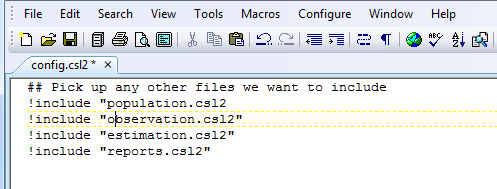
\includegraphics[scale=1]{Figures/config.png}
	\caption{\textbf{Example of using the \config~command \texttt{!include}
	 "\argument{filename}".}}\label{fig:config_file_1}
\end{figure}
%\vspace*{1mm}

The command and subcommand syntax to be used in each of these configuration sections are listed in Sections \ref{sec:population-syntax} (Population), \ref{sec:estimation-syntax} (Estimation), \ref{sec:observation-syntax} (Observation) and \ref{sec:report-syntax} (Report).

\subsubsection{Commands}\index{Commands}

\CNAME~has a range of commands that define the model structure, processes, parameters, observations, and how tasks are carried out. There are three types of commands

\begin{itemize}
\item Commands that have an argument and do not have subcommands (for example, \texttt{!include}\ \argument{\emph{filename}})
\item Commands that have a label and subcommands (for example \command{process} must have a label and has subcommands)
\item Commands that do not have either a label or argument, but have subcommands (for example \command{model})
\end{itemize}

Apart from \texttt{!include}, commands start with an \texttt{@} in column 1. Otherwise, inputs are free form. The \texttt{@} is important as it signals the start of a command block which is the basic  unit in the input files (see sub-section \ref{{sec:command-block-format}}).

Commands that have a label must have a unique label, i.e., the label cannot be used on more than one command of that type so that it can be referenced in other parts of the \config. The labels can contain alpha numeric characters, period (`.'), underscore (`\_') and dash (`-'). Labels must not contain whitespace (tabs or spaces) or other characters that are not letters, numbers, dash, period, or an underscore. For example,

{\small{\begin{verbatim}
@process NaturalMortality
or
!include MyModelSpecification.csl2
\end{verbatim}}}

\subsubsection{Subcommands}\index{Commands ! Subcommands}

\CNAME~subcommands define options and parameter values related to a particular command. Subcommands always take an argument which is one of a specific \emph{type}. The argument \emph{types} acceptable for each subcommand are defined in Section \ref{sec:syntax}, and are summarised below.

Like commands (\command{command}), subcommands and their arguments are not order specific, except that that all subcommands of a given command must appear before the next \command{command} block. \CNAME~may report an error if they are not supplied in this way. However, in some circumstances a different order may result in a valid, but unintended, set of actions, leading to possible errors in the expected results.

The argument type for a subcommand can be\index{Subcommand argument type}:

\begin{tabular}{ll}
\textbf{switch} & true/false \\
\textbf{integer}& an integer number \\
\textbf{integer vector} & a vector of integer numbers \\
\textbf{integer range} & a range of integer numbers separated by a colon, e.g. 1994:1996 is \\ & expanded to an integer vector of values (1994 1995 1996) \\
\textbf{constant} & a real number (i.e., a double) \\
\textbf{constant vector} & a vector of real numbers (i.e., a vector of doubles) \\
\textbf{estimable} & a real number that can be estimated (i.e., a double) \\
\textbf{estimable vector} & a vector of real numbers that can be estimated (i.e., a vector of doubles) \\
\textbf{addressable} & a real number that can be referenced but not estimated (i.e., an addressable double) \\
\textbf{addressable vector} & a vector of real numbers that can be referenced but not estimated (i.e., a vector of \\ & addressable doubles) \\
\textbf{string} & a categorical (string) value \\
\textbf{string vector} & a vector of categorical values.
\end{tabular}

Switches are characteristics which are either true or false. Enter \emph{true} as \argument{true} or \argument{t}, and \emph{false} as \argument{false} or \argument{f}.

Integers must be entered as whole numbers without decimal points (i.e., if \subcommand{year}\ is an integer then it is specified as \texttt{2008}, not \texttt{2008.0})

Arguments of type integer vector, constant vector, estimable vector, addressable vector, or categorical vector must contain one or more entries on a row, separated by whitespace (tabs or spaces). Arguments of type integer range must contain a colon (\texttt{:}) and no whitespace (tabs or spaces).

Parameters are defined in the population section and can be specified as estimable with the subcommand type \texttt{estimable} or \texttt{estimable vector}.  These parameters will be estimated if specified as such in the estimation section. If an estimable parameter is not specified in the estimation section it will instead be treated as a constant (or constant vector). In other words, only estimable parameters can be estimated and the parameter command must explicitly specify that the parameter is estimable with the \texttt{estimable} or \texttt{estimable vector} subcommand type. TODO: check

Parameters defined as addressable with the subcommand type \texttt{addressable} or \texttt{addressable vector} are usually derived quantities and are not directly estimable. As such, they can be referenced by various processes, or have priors and/or penalties associated with them, but they do not directly contribute to any estimation within the model. WHAT IS ADDRESSABLE????

\subsubsection{The command block format}\index{Command block format}\label{sec:command-block-format}

The command block is a basic continuous unit within the input file(s). It begin with a line that starts with the symbol \command{}, juxtaposition against a single command and followed, if required, by any unique label or argument. There is no indicator of the end of a command block. Each command block is delimited by the end of the file or the start of the next command block (which is marked by the \command{} on the first character of a line). The \texttt{!include} command is the only exception to this rule (see Section \ref{sec:general-syntax}\index{command ! include files} for details of the use of \texttt{!include}). The \texttt{!include} command can be used to include contents of another file within the scope of the command block.

Within the command block, any subcommands needed and their arguments are presented,

%\begin{multicols}{3}
%	\begin{description}
%		\item \command{command}
%		\item \subcommand{subcommand} \subcommand{argument}
%		\item \subcommand{subcommand} \subcommand{argument}
%		\item .
%		\item .
%		\item etc.
%		\item \command{command} \subcommand{argument}
%		\item \subcommand{subcommand} \subcommand{argument}
%		\item \subcommand{subcommand} \subcommand{argument}
%		\item .
%		\item .
%		\item etc.
%		\item \command{command} \subcommand{\emph{label}}
%		\item \subcommand{subcommand} \subcommand{argument}
%		\item \subcommand{subcommand} \subcommand{argument}
%		\item .
%		\item .
%		\item etc.
%		\end{description}
%\end{multicols}

Subcommands can be in any order within the command block. Command blocks can be in any order within the input files, except \texttt{\command{}model} which must be the first command block encountered by \CNAME~since this scopes the basic model dimensions (but excluding the \texttt{!include} command).
	
Blank lines are ignored, as is extra whitespace (tabs and spaces) between arguments. However, to start command block the \command{} character must be the first character on the line and must not be preceded by any whitespace. Each input file must end with a carriage return.

Commands, subcommands, and arguments in the \config s are not case sensitive. However, labels and variable values are case sensitive. On Linux, filenames and paths are case sensitive (i.e., when using \texttt{!include} \argument{\emph{filename}}, the argument \argument{\emph{filename}} will be case sensitive).


\subsubsection{\I{Commenting out lines}}\index{Comments}

Text on a line that starts with the symbol \commentline\ is considered to be a comment and is ignored. To comment out a group of commands or subcommands, use \commentline\ at the beginning of each line to be ignored.

Alternatively, to comment out an entire block or section, use \commentstart\ at the beginning of a line to start the comment block, then end the block with \commentend. All lines (including line breaks) between \commentstart\ and \commentend\ inclusive are ignored.

{\small{\begin{verbatim}
		# This line is a comment and will be ignored
		@process NaturalMortality
		m 0.2
		/*
		This block of text
		is a comment and
		will be ignored
		*/
\end{verbatim}}}

\subsubsection{How to reference parameters\label{sec:parameter-names}\index{Determining parameter names}\index{Parameter names}}

Parameters need an unique name so it can be referenced in other command blocks, e.g., specifying it to be estimated, to apply a penalty, specifying values to use in projections, making it time varying, or profiling. 

When \CNAME~processes the \config~it translates each command block and each subcommand block into a \CNAME~object, each with a unique parameter name. For commands, this parameter name is simply the command label. For subcommands, the parameter name format is one of the following:

\begin{description}
\item \texttt{command[label].subcommand} if the command has a label, or
\item \texttt{command.subcommand} if the command has no label, or
\item \texttt{command[label].subcommand\{i\}} if the command has a label and the subcommand arguments are a vector, and we are accessing the  \emph{i}th element of that vector.
\item \texttt{command[label].subcommand\{i:j\}} if the command has a label, and the subcommand arguments are a vector, and we are accessing the elements from $i$ to $j$ (inclusive) of that vector.
\end{description}

For example, the parameter name of the natural mortality rates subcommand \subcommand{m} of the command \command{process} with the label \argument{NaturalMortality} and there is a different rate for \argument{males} and \argument{females} has the form to reference both rates as a vector  is

\texttt{process[NaturalMortality].m}, but to reference just the male rate then the form is
\texttt{process[NaturalMortality].m\{male\}}.

All labels (parameter names) are user specified. As such, naming conventions are non-restrictive and can be model specific.


\subsection{\I{Reading a command block}\label{sec:Readingcommandblock}}\index{Reading\ command\ block}\index{Reading\ command\ block section}

Here, we illustrate reading a command block using two important commands, \texttt{@process} and \texttt{@estimate}.

The command \texttt{@process} specifies a process that can be used in the model. The are a fixed set of predefined processes (subroutines in C++ code). The way to identify which one is by the \texttt{type} subcommand. Processes can take one or more parameters and some will need other data to be applied too. Some parameters are mandatory and others can take a default value if they are not specified.
We have categories male and female, and two fisheries, line and pot. The command block starts with a\textit{@process}:

{\small{\begin{verbatim}
@process Fishing
type mortality_instantaneous
\end{verbatim}}}

This sets up a process block using the \textit{mortality\_instantaneous}~ process which simultaneously depletes the population by natural mortality and from two types of fishing. Its label is \textit{Fishing}.

Next we specify the values for natural mortality (\textit{m}) an argument to this process, to 0.17 and specify that fisheries acts on all categories. Note there are two values for natural mortality, one for each sex. The parameters \textit{m} can be estimated, if required. The command block fragment:

{\small{\begin{verbatim}
m 0.17 0.17   # natural mortality  for each category
relative_m_by_age One One # natural mortality multiplier
categories *  # fishing acts on all categories ("*" shorthand for male female)
\end{verbatim}}}

Catches are supplied via a \textit{table} format using three columns: year and two for the fisheries, one for each, which take the labels \textit{line} and \textit{pot}. Column names are on the first line of the table and these columns can be in any order,

{\small{\begin{verbatim}
#catches
table catch         # define catches by fishery in table format
year line pot       #names columns so can identity catch for each fishery
2000 1000 2000      # catches by year
2001 500  1000
2002 1000 5000
end_table           # end of table marker
\end{verbatim}}}

Other information needed are supplied in the methods table which has a fixed number of columns (again these can be in any order), one for each piece of information needed to model a fishery. The method column defines the fishery name which is used in the catch table and also in other observations like age composition from that fishery. The categories that the fishery operates on (all in this case, but it could be just males for one and females for the other) are in the category column, the fishing selectivity to be used is given as a selectivity block name which is define somewhere else in the files, \textit{u\_max} is the maximum exploitation rate in any year that is allowed, next comes the time step the fishing operates in, and lastly the block name of a penalty function that is used to penalise estimable parameter values that result in the supplied catch not being caught. Again, the penalty block is define elsewhere in the files. After the row with the column names, there follows one row for each fishery:

{\small{\begin{verbatim}
table method        # supply arguments and name selectivity etc
method  	category 	selectivity 	u_max 	time_step 		penalty
pot        	*  	       potFSel		   0.7 			1 	CatchMustBeTaken1
line     	*  	      lineFSel 	    0.7 			1 	CatchMustBeTaken1
end_table
\end{verbatim}}}

To estimate natural mortality, you need to supply an \textit{@estimate} block with a reference name back to \textit{m} in the \textit{Fishing} block. For \textit{@estimate}, \textit{type} specifies the prior to be used in the estimation, which in this case is a normal distribution:

{\small{\begin{verbatim}
@estimate estimate.m
type normal normal
parameter process[fishing].m  #
    \*Fishing is unique amongst the @process command blocks
    so     this defines the unique reference to the parameter m
    *\

mu  0.2 0.2   #argument to prior = mean
sd  0.02 0.02 #another argument to the prior = standard deviation
\end{verbatim}}}

Note that there are two \textit{m}s, one for each sex, so there has to be two priors. The \textit{\@estiamte} label \textit{estimate.m} is often redundant, but it may be needed, e.g., in a transformation command block.

To estimate a common \textit{m} over both sexes, we estimate one \textit{m}, say male, and use the \textit{same} subcommand to apply the same value to the female \textit{m},

{\small{\begin{verbatim}
@estimate estimate.m
type normal 
parameter process[fishing].m{1}  #male M since males are first in the category order
same process[fishing].m{2}       #{} is used to index one or more elements in a vector
mu  0.2    #argument to prior = mean
sd  0.02 #another argument to the prior = standard deviation
\end{verbatim}}}

There are section detailing the equations involve and a separate syntax section that gives the possible \texttt{type}s and their subcommands.

Note that the syntax sections are auto-generated from the code base (from the class constructors) so they give the definitive set of subcommands and their names. 

\subsection{\I{Single-stepping \CNAME~}\label{sec:SingleStepping}}\index{Single\_stepping}\index{single\_stepping section}

TODO: move this section to somewhere else

Single-stepping means \CNAME~can 'pause' after each year in the annual cycle during a model run, write reports, then wait and process user input of updated estimable parameters for the next year (see the command line argument \texttt{ -{}-single-step}).

This enables \CNAME~to implement models for management simulations or scenarios that require feedback and can be used, for example, in operational management procedures (OMPs). The single-stepping process can be automated using \R, so that \CNAME~may be used with \R\ to update input harvest values (e.g., catches from a fishery in a fisheries model) to evaluate a particular harvest control rule.

\subsection{\CNAME~exit status values\index{Exit status value}}

When \CNAME~is run, it will complete its task successfully or output errors. \CNAME~will return a single exit status value 'completed' to the standard output. Error messages will be printed to the console. When input file configuration errors are found, \CNAME~will print error messages, along with the associated filename(s) and line number(s) where the errors were identified, for example,

{\small{\begin{verbatim}
	#1: At line 15 in Reports.csl2: Parameter '{' is not supported
\end{verbatim}}}
